\section{Summary of results and submission}
%\label{seq:resultsubmission}

Once we have selected the best $model$ of the whole human \ttt{Hgb} and obtained good validation scores from \emringer, \molprobity and other validation programs, and we have checked that we have the whole volume density modeled, we are ready to submit the electron density map and its atomic interpretation to public databases and to make public our results.\\

\subsection*{Submission to public databases}

Although submission of cryoEM maps and derived atomic structures to databases has to be done by direct online request (\url{https://deposit-pdbe.wwpdb.org/deposition/}), \scipion may contribute to organize the submission records. The protocol \scommand{export to EMDB} allows to perform this task (Appendix \ref{app:exportToEMDB}). By using this protocol we can save the files that you have/want to submit to databases in a labelled folder and in the appropriate format. \ffigure{fig:scipion_workflow_submission} details the protocols of the modeling \scipion workflow involved in this task.

 \begin{figure}[H]
  \centering 
  \captionsetup{width=.9\linewidth} 
  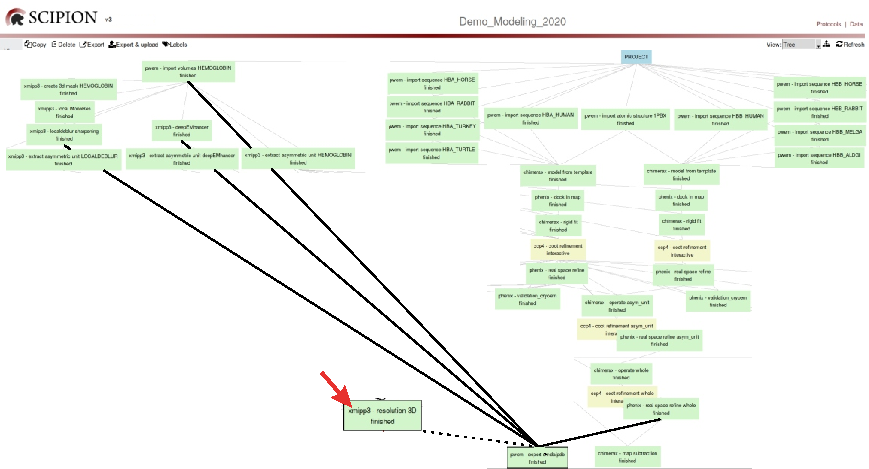
\includegraphics[width=1\textwidth]{Images/Fig78}
  \caption{\scipion framework detailing the workflow to submit \cryoEM results to databases.}
  \label{fig:scipion_workflow_submission}
  \end{figure}

When you submit the \iii{map} and the \iii{model} of a \cryoem experiment, besides these two records, an image of the \iii{map} is also mandatory to submit. Other maps, such as half maps or postprocessing-sharpening maps, as well as maks, are also recommended to submit. In addition, the \ttt{FSC} file is strongly encouraged. As you can see in \ffigure{fig:scipion_workflow_submission}, we can provide directly from the workflow the \iii{map} and the \iii{model}, as well as the two sharpening maps. The \iii{map} image can be attached from a file. We lack, however, from the \ttt{FSC} file, since the \ttt{FSC} file is usually generated during the \iii{map} reconstruction process starting from the half maps, for example with the \scommand{xmipp3 - resolution 3D} protocol(\ffigure{fig:scipion_workflow_submission}, red arrow). To compute the \ttt{FSC} file we could download the half maps from the database 
(\url{https://www.ebi.ac.uk/pdbe/entry/emdb/EMD-3488/index}) selecting the \ttt{zip} Bundle (\ffigure{fig:export_to_EMDB_protocol_1} (red arrow)).

 \begin{figure}[H]
  \centering 
  \captionsetup{width=.9\linewidth} 
  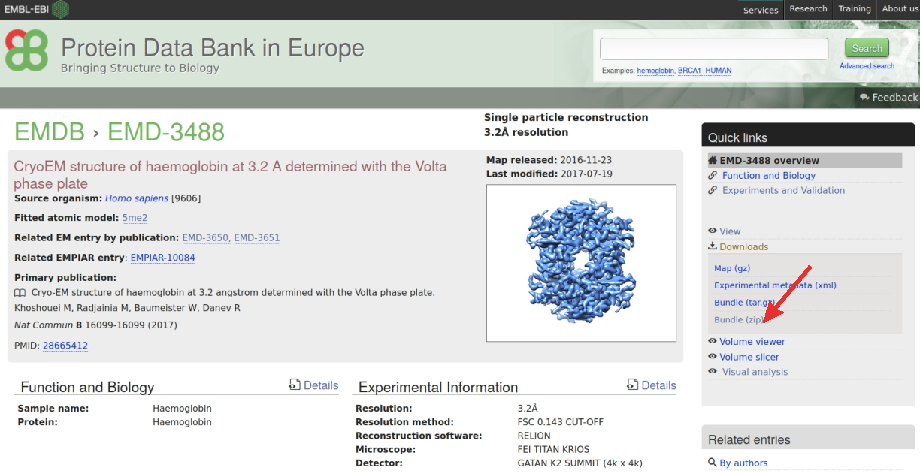
\includegraphics[width=0.9\textwidth]{Images/Fig77}
  \caption{\ttt{EMDB} entry \ttt{3488} in \ttt{PDBe}}
  \label{fig:export_to_EMDB_protocol_1}
  \end{figure}

The \ttt{zip} folder contains the \ttt{FSC} file (\ttt{emd\_3488\_fsc.xml}) and the \iii{map} image (\ttt{emd\_3488.png}) but, unfortunately, lacks of half maps. Then, you can use any two half maps and compute the \ttt{FSC} file, just to submit it with the rest of the files.
  
To save all the relevant files in a single labelled folder, open the \scommand{export to EMDB} protocol (\ffigure{fig:export_to_EMDB_protocol} (1)), and complete the form with the \scipion elements to export: \ttt{Main map} (2), \ttt{Additional maps: ``Yes''} (3), the two sharpened maps as additional maps (4), the \ttt{FSC} file if you count on it (5), \ttt{Atomic structure} (6) and \ttt{Image} (7), previously saved in a known folder. Then, write the name of the exportation directory path, or find it with the browser on the right. All submission files will be saved in the \ttt{directory} selected (8). A directory name related with the submission (number, date, project,...) is recommended. 
 
 \begin{figure}[H]
  \centering 
  \captionsetup{width=.7\linewidth} 
  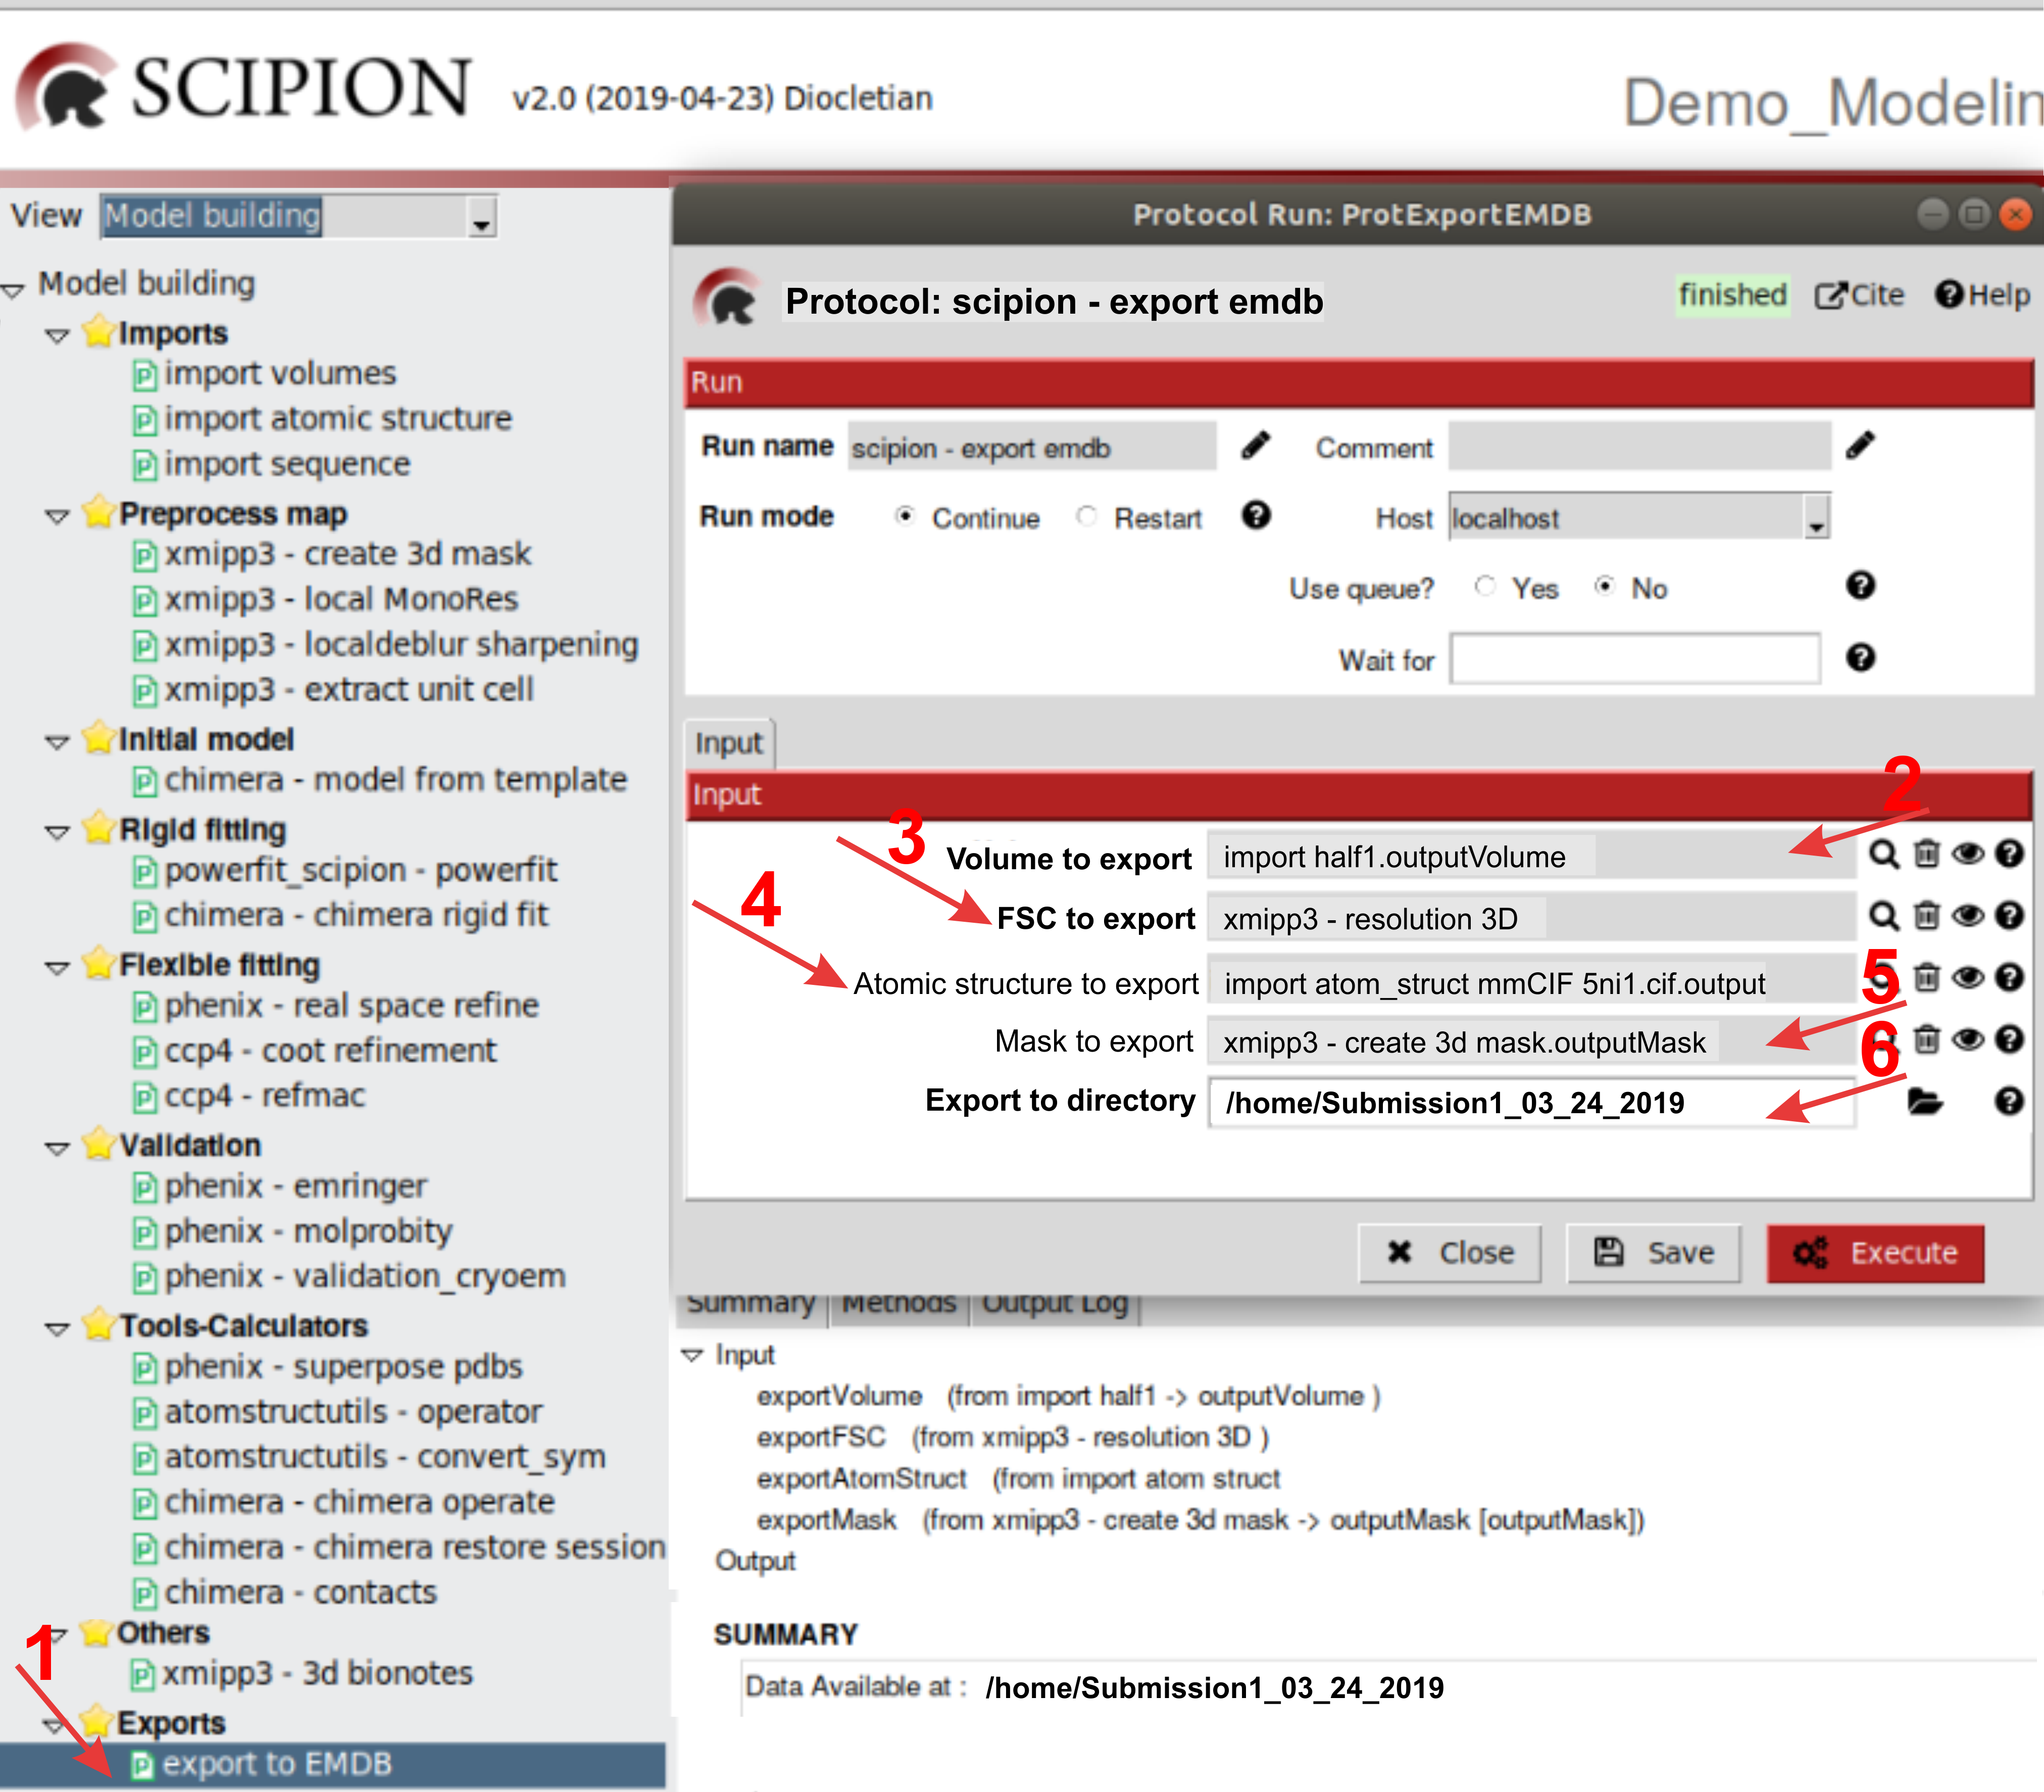
\includegraphics[width=0.9\textwidth]{Images/Fig45}
  \caption{Saving files for submission to EMDB with protocol \scommand{export to EMDB}}
  \label{fig:export_to_EMDB_protocol}
  \end{figure}
  
After executing the protocol (9), you can check that all files are saved in the given directory. No additional visualization tools have been included in this protocol. 

\subsection*{Publication of results}

Since the atomic interpretation of a certain macromolecule will be probably the starting point of relevant mechanistic or biomedical studies, summaring and organizing our results constitutes the first step to draw the conclusions that will be made public by journals and talks. Many different questions can be posed based on the atomic structure. Here we are wondering about interactions among members of the macromolecule. To answer this question we have included in \scipion the protocol \scommand{chimerax - contacts} to identify the residues involved in contacts between any couple of interacting molecules. ``contacts'' involve atoms within  favorable interaction distances. Unfavourable contacts or severe clashes, in which atoms are too close together, although discarded by default in the final list of `contacts'', may also be shown by using appropriate advanced parameters, as you can see in Appendix \ref{app:chimeraContactsProtocol}. \\

As an example, in this tutorial we are going to learn how to get atom contacts of human haemoglobin \ttt{metHgb} atomic structure \ttt{5NI1}, associated to the starting map \ttt{EMD-3488}. This structure was already downloaded from \ttt{PDB} by using the protocol \scommand{import atomic structure} (\ffigure{fig:workflows_contacts} (1)). According to the aim of the analysis, two possible scenarios and the respective workflows can be considered to compute contacts: a) infering all contacts between any couple of members of the whole macromolecule (\ffigure{fig:workflows_contacts} (3)); b) infering all contacts between any couple of members of the asymmetric unit, and between one member of the asymmetric unit and another component from a neighbor asymmetric unit (\ffigure{fig:workflows_contacts} (5)). 

        \begin{figure}[H]
            \centering 
            \captionsetup{width=.9\linewidth} 
            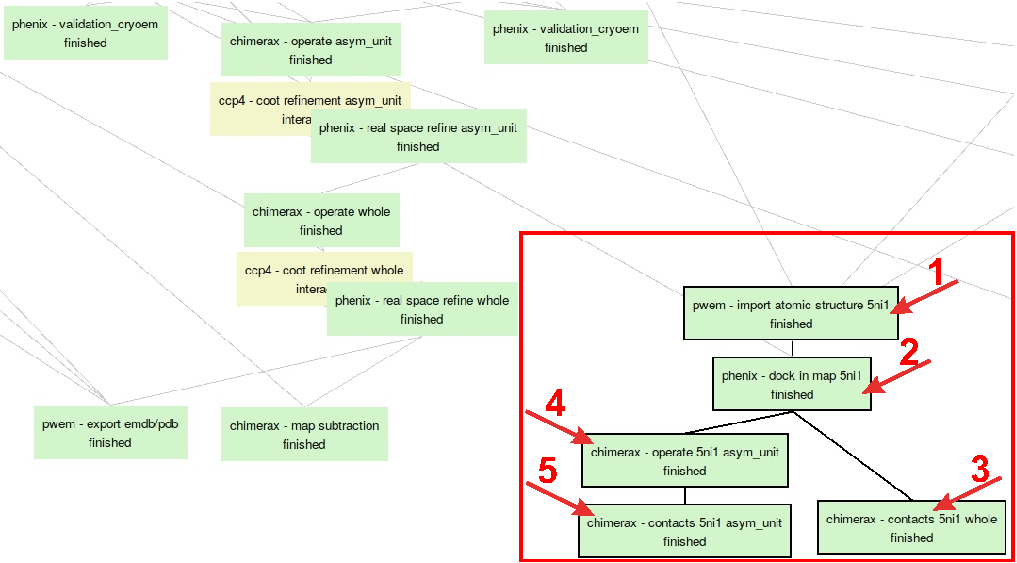
\includegraphics[width=0.9\textwidth]{Images/Fig46}
            \caption{\scipion workflows inside the red box to get contacts between any two chains of a macromolecule (3) and between any two chains of the asymmetric unit, and between any chain of the asymmetric unit and a chain of a neighbor asymmetric unit (5).}
            \label{fig:workflows_contacts}
        \end{figure}
        
Since the penultimate step of the second workflow (\ffigure{fig:workflows_contacts} (4)) requires applying symmetry, we are going to start moving the structure to match its symmetry center to the origin of coordinates using the protocol \scommand{phenix - dock in map} as we did previously (\ffigure{fig:dockInMap_protocol}), including the whole starting map of the human \ttt{metHgb} and the imported atomic structure \ttt{5NI1} as \ttt{Input map} and \ttt{Input atom structure}, respectively.\\

Secondly, we are going to extract the structure of the asymmetric unit of the docked \ttt{5NI1} structure using the protocol \scommand{chimerax - operator} as it is indicated in \ffigure{fig:workflows_contacts} (4). Complete the protocol form including the last docked structure \ttt{5NI1} as \ttt{Atomic structure}. After executing the protocol, the \chimera graphics window will open. You can select and save the atomic structure of the map asymmetric unit writing in the \chimera command line:\\
 \\
 \ttt{select \#2/A,B}\\
 \ttt{save /tmp/chainAB.cif format mmcif models \#2 selectedOnly true}\\
 \ttt{open /tmp/chainAB.cif}\\
 \ttt{scipionwrite \#3 chainAB\_}\\
 \ttt{exit}\\

    \begin{itemize}
    
\item CASE A: Contacts between any couple of members of the whole macromolecule (\ffigure{fig:workflows_contacts} (3)):\\
 This option allows to get all contacts between all couples of members of the macromolecule. In the case of the human \ttt{metHgb} we have depicted all those possible contacts in the \ffigure{fig:schema_contacts} (A).
 
 \begin{figure}[H]
            \centering 
            \captionsetup{width=.9\linewidth} 
            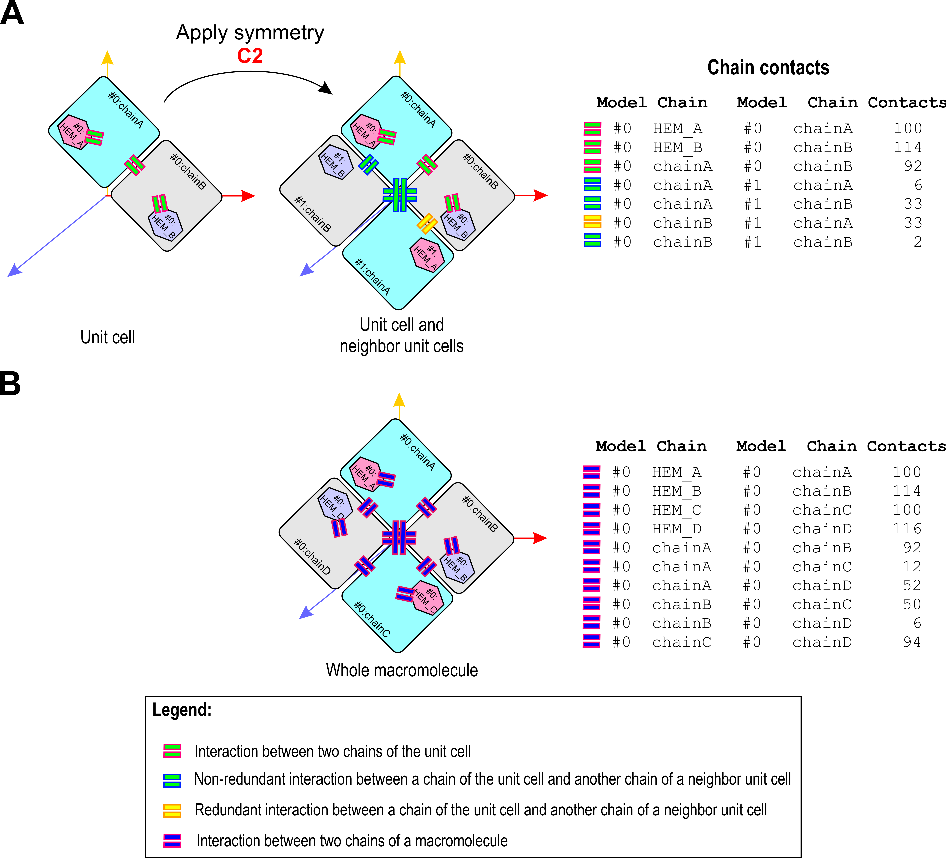
\includegraphics[width=0.9\textwidth]{Images/Fig49}
            \caption{Schema of the human haemoglobin \ttt{metHgb} showing protein contacts between couples of chains of the whole macromolecule (A) and contacts obtained by applying symmetry to the asymmetric unit (B).}
            \label{fig:schema_contacts}
        \end{figure}
 
 
 The protocol \scommand{chimerax - contacts} can be used to obtain the contacts depicted. Open this protocol (\ffigure{fig:contacts_unit cell} (1)) and fill in the first \ttt{Input} (2) in which no symmetry will be applied. Include the docked \ttt{5NI1} structure (4) as \ttt{Atomic structure}. Use the wizard on the right to label the molecule chains (5) as they appear in the adjacent window, and execute the protocol. 
 
  \begin{figure}[H]
            \centering 
            \captionsetup{width=.9\linewidth} 
            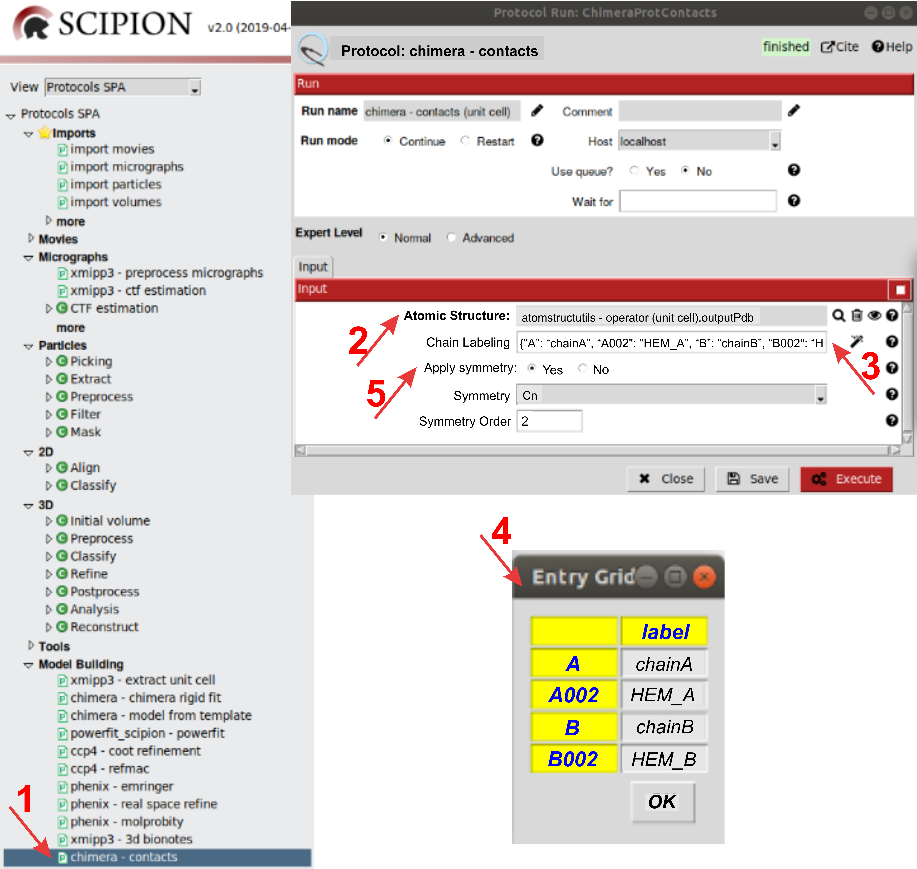
\includegraphics[width=0.9\textwidth]{Images/Fig50}
            \caption{Filling in the \scommand{chimerax - contacts} protocol form with two different inputs: (2) to get atom contacts between couples of chains within the whole \ttt{metHgb}; (3) to get contacts between any couple of chains within the asymmetric unit, and ``non-redundant`` contacts between the asymmetric unit and another chain of a neighbor asymmetric unit of the human haemoglobin \ttt{metHgb}.}
            \label{fig:contacts_unit cell}
        \end{figure}
        
After executing the protocol, all atom contacts between the couples of proteins indicated in \ffigure{fig:schema_contacts} (A) can be visualized by clicking \scommand{Analyze Results} (\ffigure{fig:contacts_results} (A)).
 
 \begin{figure}[H]
            \centering 
            \captionsetup{width=.9\linewidth} 
            \includegraphics[width=0.9\textwidth]{Images/Fig52}
            \caption{(A) Display of results of atom contacts between couples of chains within the whole \ttt{metHgb}; (B) Display of results of atom contacts between couples of chains within the asymmetric unit, and ''non-redundant`` contacts between a chain of the asymmetric unit and another chain from a neighbor asymmetric unit of the human haemoglobin \ttt{metHgb}.}
            \label{fig:contacts_results}
        \end{figure}

The viewer window of the protocol \chimera \ttt{contacts} display different results (\ffigure{fig:contacts_results}(A)):
    \begin{itemize}
    \item \ttt{3D Visualization} box: Final atomic structure considered to compute contacts that can be visualized with \chimera. Press the eye (1) to open the structure shown on the right.
    \item \ttt{Interacting chains} box: Summary list of all interacting chains, similar to the list shown on the right of the \ffigure{fig:schema_contacts} (A). Press the eye to open it (2).
    \item \ttt{Contacts between interacting chains} box: In addition to the possibility of changing the order of the interacting chains in the display, as well as the maximal distance between residues to group them, this box allows to select couples of interacting chains (4) and inspect in detail the contacts between them pressing the eye on the right (3).
    \end{itemize}
 
 
 
\item CASE B: Contacts between any couple of members of the asymmetric unit and ''non-redundant`` contacts between one member of the asymmetric unit and another one from the neighbor asymmetric unit (\ffigure{fig:workflows_contacts} (5)). This second asymmetric unit has been obtained by applying symmetry with the protocol \scommand{chimerax - contacts}. Then, ``non-redundant'' interaction means any interaction that can not be inferred by symmetry. The  \ffigure{fig:schema_contacts} (B) shows the total number of interactions of our example. The interactions between the chain \ttt{B} of the asymmetric unit (model \ttt{\#1.1}) and the chain \ttt{A} of the neighbor asymmetric unit (model \ttt{\#1.2}) are symmetric to the interactions between chain \ttt{A} of the asymmetric unit (model \ttt{\#1.1}) and chain \ttt{B} of the neighbor asymmetric unit (model \ttt{\#1.2}). Since those interactions can thus be inferred by symmetry, they are ``redundant'' and are absent of the final list of contacts.\\  
       
Similarly to the case A, the protocol form has to be open (\ffigure{fig:contacts_unit cell} (1) ) and completed as indicated in the second \ttt{Input} (3). Include the asymmetric unit structure saved with the protocol \chimera \ttt{operate} (6), use the wizard on the right (7) to label the chains as it is shown on the right and, finally, include the respective type of symmetry of the human \ttt{metHgb} (8).\\ 
        
Like in the case A, after executing the protocol all non-redundant atom contacts between any couple of proteins indicated in \ffigure{fig:schema_contacts} (B) can be visualized by clicking \scommand{Analyze Results} (\ffigure{fig:contacts_results} (B)). Besides the lower number of contacts displayed, remark that a relevant difference between the results of the case A and the case B is the final atomic structure visualized with \chimera, which discriminates between the starting asymmetric unit and the second one generated by symmetry.\\
 
\\
\ttt{Note}: This second possibility of getting protein contacts observed in the case B is extremely useful when you have a big asymmetric unit, for example of a virus, and you are interested in contacts among proteins within the asymmetric unit and with other adjacent asymmetric units.
\end{itemize}















\begin{comment}
Besides this preprocesing step, and because protocol \scommand{chimerax - contacts} only computes contacts between independent chains and not whitin the same chain, an additional preprocessing step has to be performed to separate \ttt{HEM} groups in independent chains to get contacts between proteins and ligands (\ttt{HEM} groups).

\begin{itemize}
 \item Preprocessing:\
 In this step, the macromolecule constituted by four chains, each one containing a \ttt{HEM} group, will be transformed in a molecule of eight independent chains, four proteins and four \ttt{HEM} groups, with its symmetry center in the origin of coordinates. Two protocols already mentioned before are going to be used to move the structure and to extract proteins and ligands of the starting atomic structure, \scommand{atomstructutils - operator} protocol (Appendix \ref{app:atomStructUtilsOperatorProtocol}), and the protocol \scommand{chimerax - operate} (Appendix \ref{app:chimeraOperate}).\
    \begin{itemize}
    \item Matching between symmetry center of human haemoglobin \ttt{metHgb} atomic structure \ttt{5NI1} and origin of coordinates (upper brown box in A and B workflows of \ffigure{fig:workflows_contacts}):\\
    Open the protocol \scommand{chimerax - operate} and complete the form with \ttt{5NI1} as \ttt{Atomic structure} and the structure of the \ttt{Hgb} obtained by \scommand{phenix - real space refine} protocol as \ttt{Other atomic structures}. When the \chimera graphics window opens, write in the command line:\\
    \\
    \ttt{matchmaker \#2 to \#3}\\
    \\Save the structure \ttt{5NI1} in its new location with the command line:\\
    \\
    \ttt{scipionwrite \#3 prefix 5ni1\_\origin_}\\
    \\
    \ttt{exit}
        
    To visualize the new position of the atomic structure \ttt{5NI1}, open the \chimera viewer by clicking \scommand{Analyze Results}.

    \item Independent extraction of aminoacid chains A, B, C and D (dark blue boxes in workflows A and B of \ffigure{fig:workflows_contacts}):\\
    Open the protocol \scommand{atomstructutils - operator} (\ffigure{fig:atomStructUtils_extractChain} (1)) and fill in the form with the atomic structure (2) and the operation to accomplish, in this case chain extraction (3), to extract chain A (4), that can be selected with the help of the wizard on the right. The default values of starting (5) and ending (6) residues allow to extract the whole chain. Then, execute the protocol. The extracted A chain can be visualized with \chimera by clicking \scommand{Analyze Results}. Repeat this process to extract, one by one, chains B, C and D.
    
     \ttt{sel \#2/C,D}\\
     \ttt{del sel}\\
     \ttt{scipionwrite \#2 prefix 5ni1\_asym\_unit\_}\\
    
        \begin{figure}[H]
            \centering 
            \captionsetup{width=.7\linewidth} 
            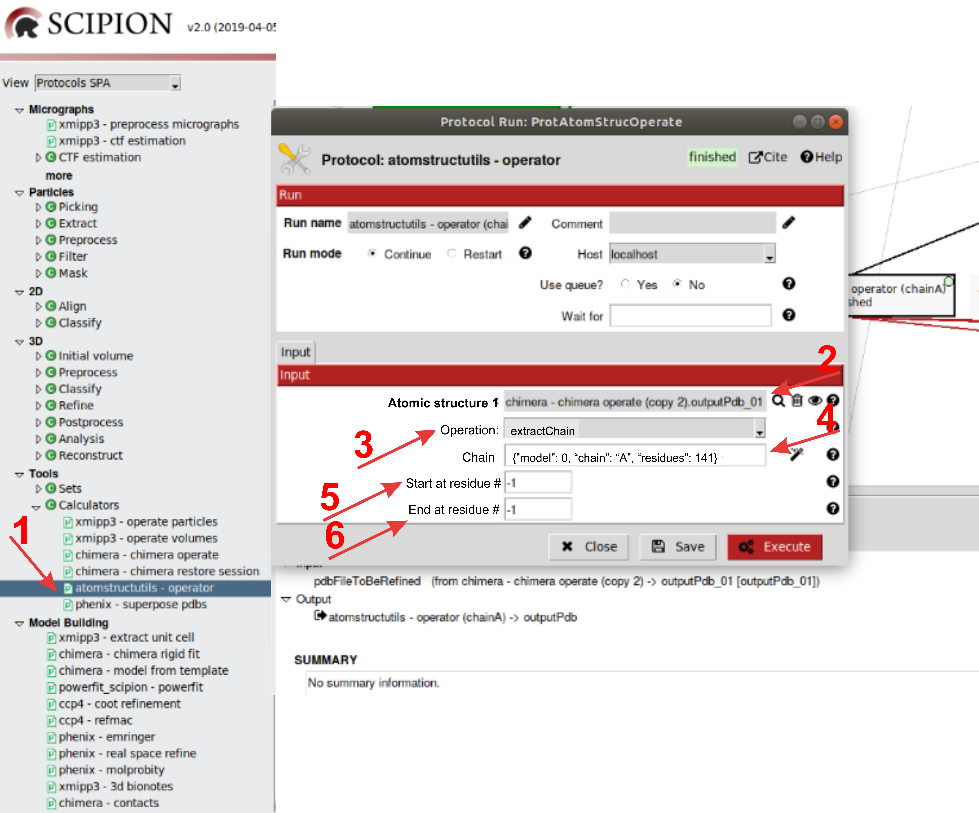
\includegraphics[width=0.85\textwidth]{Images/Fig47}
            \caption{Extraction of chain A of human haemoglobin \ttt{metHgb} with protocol \scommand{atomstructutils - operator}.}
            \label{fig:atomStructUtils_extractChain}
        \end{figure}
    
    \item Independent extraction of \ttt{HEM} groups associated to each aminoacid chain from human haemoglobin \ttt{metHgb} atomic structure \ttt{5NI1} (lower brown box in workflows A and B of \ffigure{fig:workflows_contacts}):\
    Open the protocol \scommand{chimerax - operate} and complete the form with the atomic structure \ttt{5NI1} and follow these intructions when \chimera graphics window opens:
        \begin{itemize}
        \item Selection of \ttt{HEM} groups:\\
            \chimera main menu: \ttt{Select -> Residue -> HEM}
        \item Selection of every element except \ttt{HEM} groups:\\
            \chimera main menu: \ttt{Select -> Invert (selected models)}
        \item Remove every element except \ttt{HEM} groups:\\
            \chimera command line: \ttt{del sel}
        \item Split \ttt{HEM} groups in four independent chains:\\
            \chimera command line: \ttt{split}
        \item Save \ttt{HEM} groups one by one as models 1.1 to 1.4:\\ 
            \chimera command line: \ttt{scipionwrite \#1.1 prefix HEM\_A\_}\\
            \chimera command line: \ttt{scipionwrite \#1.2 prefix HEM\_B\_}\\
            \chimera command line: \ttt{scipionwrite \#1.3 prefix HEM\_C\_}\\
            \chimera command line: \ttt{scipionwrite \#1.4 prefix HEM\_D\_}
        \end{itemize}
        
    Remark that, although \scommand{chimerax - operate} protocol might also be used to extract independently aminoacid chains A, B, C and D, we have chosen the protocol \scommand{atomstructutils - operator} to exclude water molecules associated to aminoacid chains.
    
    \item Reconstruction of the unit cell of the human haemoglobin \ttt{metHgb} atomic structure (\ffigure{fig:workflows_contacts} (A; 1)):\
    Protocol \scommand{atomstructutils - operator} will be used to perform this task by selecting, in this case, \ttt{addChain} as operation option (\ffigure{fig:atomstructutils_addChain_1} (A; 2)).
    
        \begin{figure}[H]
            \centering 
            \captionsetup{width=.7\linewidth} 
            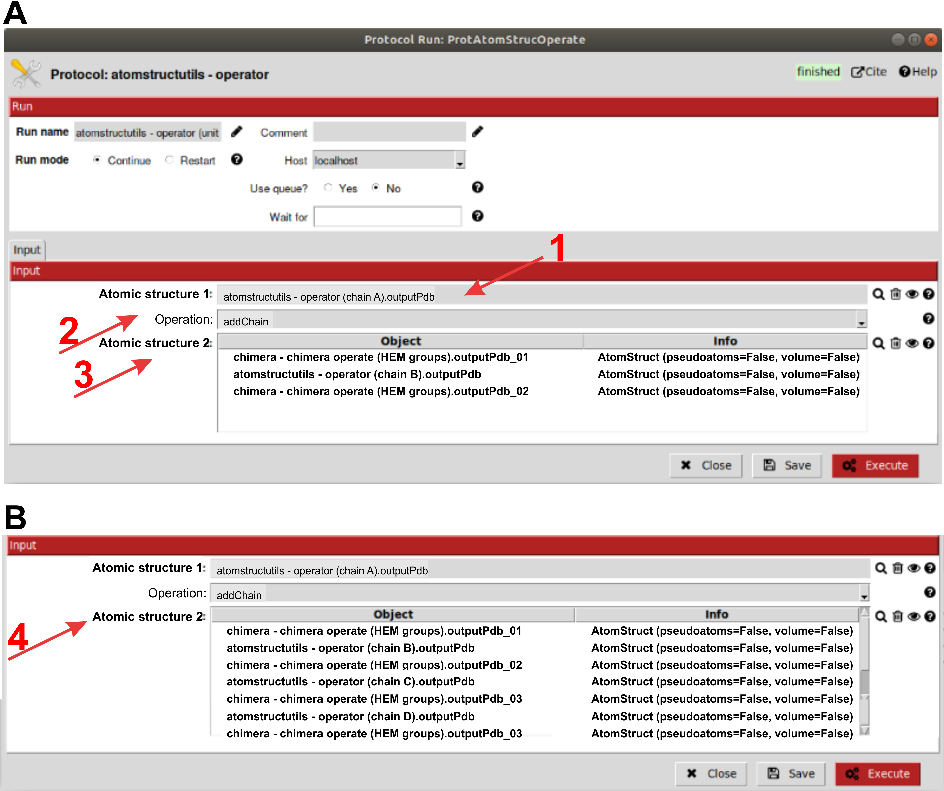
\includegraphics[width=0.85\textwidth]{Images/Fig48}
            \caption{Completing the protocol form to reconstruct the map asymmetric unit (A) and the whole macromolecule (B) of the human haemoglobin \ttt{metHgb} with protocol \scommand{atomstructutils - operator}.}
            \label{fig:atomstructutils_addChain_1}
        \end{figure}
        
    To the previously extracted chain A (\ffigure{fig:atomstructutils_addChain_1} (A; 1)) we add (2) its respective \ttt{HEM} group, as well as chain B and its respective \ttt{HEM} group (3). To visualize the reconstructed unit cell, open the \chimera viewer by clicking \scommand{Analyze Results}. Remark that the symmetry center is equal to the origin of coordinates and this allows to regenerate the whole molecule by applying symmetry (see Appendix \ref{app:chimeraContactsProtocol} for a deeper explanation).
    
    \item Reconstruction of the whole macromolecule of the human haemoglobin \ttt{metHgb} atomic structure (\ffigure{fig:workflows_contacts} (B; 3)):\
    Analogously to the unit cell, protocol \scommand{atomstructutils - operator} will be used to build the whole macromolecule. In this case, besides adding to chain A (\ffigure{fig:atomstructutils_addChain_1} (B; 4)) the same elements that we added to get the unit cell, we have added chains C and D and their respective \ttt{HEM} groups.\\
        
    Again, the reconstructed whole macromolecule can also be visualized with \chimera by clicking \scommand{Analyze Results}. The symmetry center of the macromolecule is set in the center of coordinates. Unlike with the unit cell, no symmetry will be applied to get contacts among chains. The location of the macromolecule is thus irrelevant to analyze the contacts.
    \end{itemize}
 
 \item CASE A: Contacts between any couple of members of the unit cell and  between one       member of the unit cell and another one from a neighbor unit cell (\ffigure{fig:workflows_contacts} (A; 2)):\\
 This option allows to get all contacts between all couples of members of the unit cell and all ``non-redundant'' interactions between a chain of the unit cell and a chain of a neighbor unit cell by using the protocol \scommand{chimera contacts}. ``non-redundant'' interaction means any interaction that can not be inferred by symmetry. \ffigure{fig:schema_contacts} (A) shows the total number of interactions of our example including ``redundant'' interactions. The 33 interactions between the chain \ttt{B} of the unit cell (model \ttt{\#0}) and the chain \ttt{A} of the neighbor unit cell (model \ttt{\#1}) are symmetric to the interactions between chain \ttt{A} of the unit cell (model \ttt{\#0}) and chain \ttt{B} of the neighbor unit cell (model \ttt{\#1}). Since those interactions can thus be inferred by symmetry, they are ``redundant'' and will be absent of the final list of contacts.  
    
        \begin{figure}[H]
            \centering 
            \captionsetup{width=.7\linewidth} 
            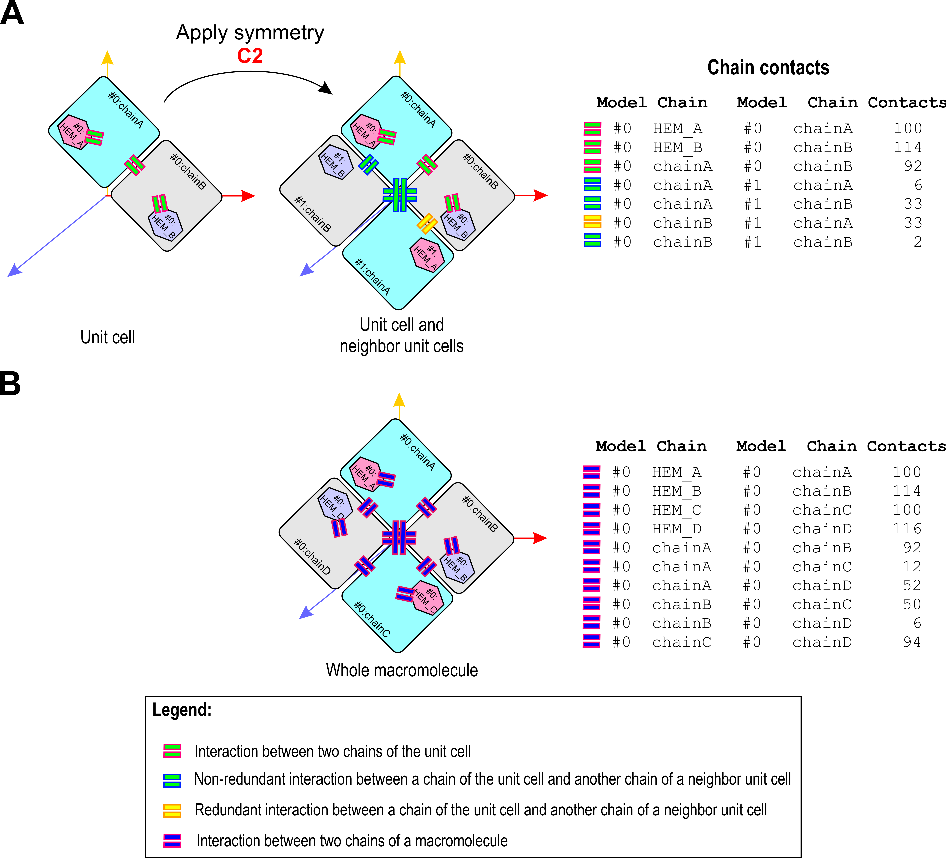
\includegraphics[width=0.85\textwidth]{Images/Fig49}
            \caption{Schema of the human haemoglobin \ttt{metHgb} showing protein contacts obtained by applying symmetry to the unit cell (A), and contacts between couples of chains of the whole macromolecule (B).}
            \label{fig:schema_contacts}
        \end{figure}
        
This list of protein contacts was obtained in \scipion by running the protocol \scommand{chimera contacts}. The protocol form opened (\ffigure{fig:contacts_unit cell} (1)) is completed with the input atomic structure of the human haemoglobin \ttt{metHgb} unit cell (2) and labelled each structure chain (3). With this labelling, a specific label is assigned to each chain in order to group chains with the same label (see Appendix \ref{app:chimeraContactsProtocol} for details). Since in this particular case we do not want to group chains, independent labels will be assigned to each chain ((\ffigure{fig:contacts_unit cell} (4)) with the help of the wizard (3). To apply symmetry to the input unit cell, we select \ttt{Yes} to the Apply Symmetry option (5). A panel with the different types of symmetry will be displayed to chose our specific Symmetry, cyclic (Cn) in our case, and our Symmetry Order (2). 

        \begin{figure}[H]
            \centering 
            \captionsetup{width=.7\linewidth} 
            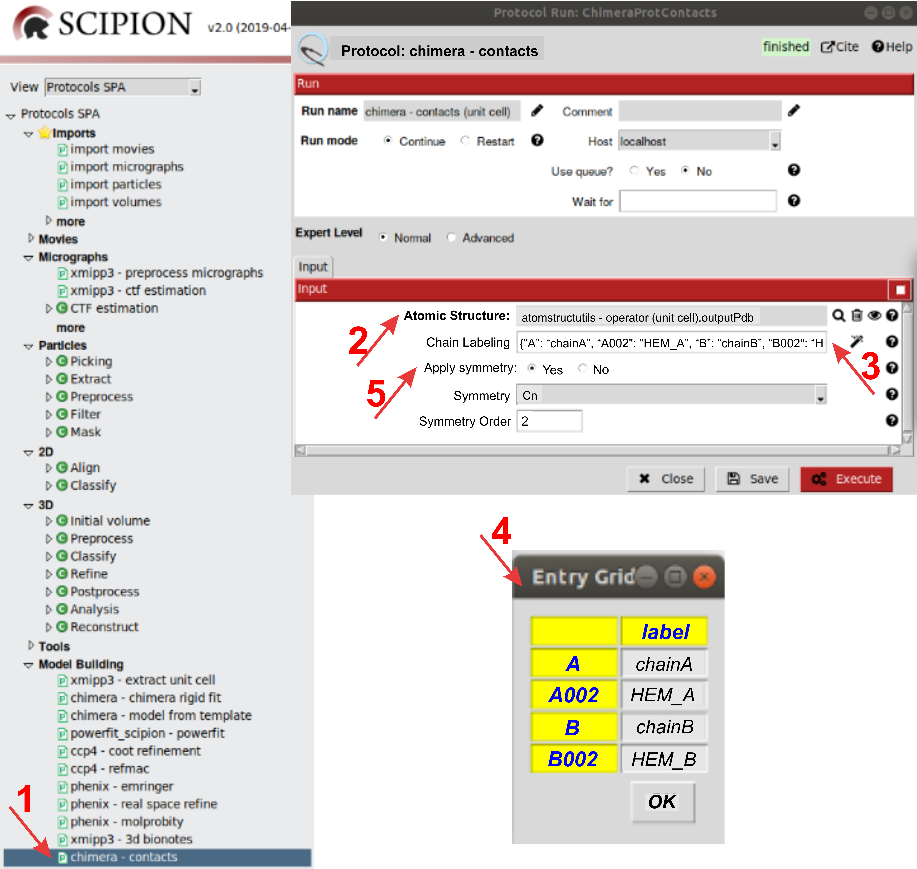
\includegraphics[width=0.85\textwidth]{Images/Fig50}
            \caption{Filling in the \scommand{chimerax - contacts} protocol form to get atom contacts between couples of chains within the unit cell, and ``non-redundant`` contacts between a chain of the unit cell and another chain from a neighbor unit cell of the human haemoglobin \ttt{metHgb}.}
            \label{fig:contacts_unit cell}
        \end{figure}
  
 After executing the protocol, non-redundant atom contacts between the couples of proteins indicated in \ffigure{fig:schema_contacts} (A) can be visualized by clicking \scommand{Analyze Results} (\ffigure{fig:contacts_results} (A)).
 
        \begin{figure}[H]
            \centering 
            \captionsetup{width=.7\linewidth} 
            \includegraphics[width=0.85\textwidth]{Images/Fig52}
            \caption{(A) Display of results of atom contacts between couples of chains within the unit cell, and ''non-redundant`` contacts between a chain of the unit cell and another chain from a neighbor unit cell, of the human haemoglobin \ttt{metHgb}. (B) \chimera view of input (blue) and symmetrical (pink) unit cells. (C) Summary of atom contacts between residues of input unit cell chain A and its respective \ttt{HEM} group. (D) Detail of the 21 atom contacts between the residue \ttt{His87} of chain A and its respective \ttt{HEM} group (yellow lines).}
            \label{fig:contacts_results}
        \end{figure}
        
  Models can be visualized with \chimera (\ffigure{fig:contacts_results} (A; 1)). (B) shows the model of the initial unit cell and the new unit cell, generated by symmetry regarding the origin of coordinates. This structure, combining both models, serves as starting point to compute atom contacts. The list that contains the six couples of interacting chains can be displayed in \ffigure{fig:contacts_results} (A; 2), and each one of these interactions can be selected in \ffigure{fig:contacts_results} (A; 3). A text list details all atom contacts between the residues of chain A and its respective \ttt{HEM} group (A; 4). The higher number of atom contacts (21) involves the \ttt{His87} residue (framed in red). A detail of this interaction is shown in \ffigure{fig:contacts_results} (D). Analogously, the rest of atom contacts can be observed by selecting each one of the five remaining couples of interacting proteins.
  
 \item CASE B: Contacts between any couple of members of the whole macromolecule (\ffigure{fig:workflows_contacts} (B; 4)):\\
 This option allows to get all contacts between all couples of members of the macromolecule (\ffigure{fig:schema_contacts} (B)) by using the protocol \scommand{chimera contacts}. Similarly to case A, the protocol form has to be completed with the Atomic Structure (\ffigure{fig:contacts_whole_macromolecule} (1)), and the Chain Labelling (3) with help of the wizard (2). Unlike in case A, the option \ttt{No} in Apply symmetry has to be selected in this case (4). 
 
        \begin{figure}[H]
            \centering 
            \captionsetup{width=.7\linewidth} 
            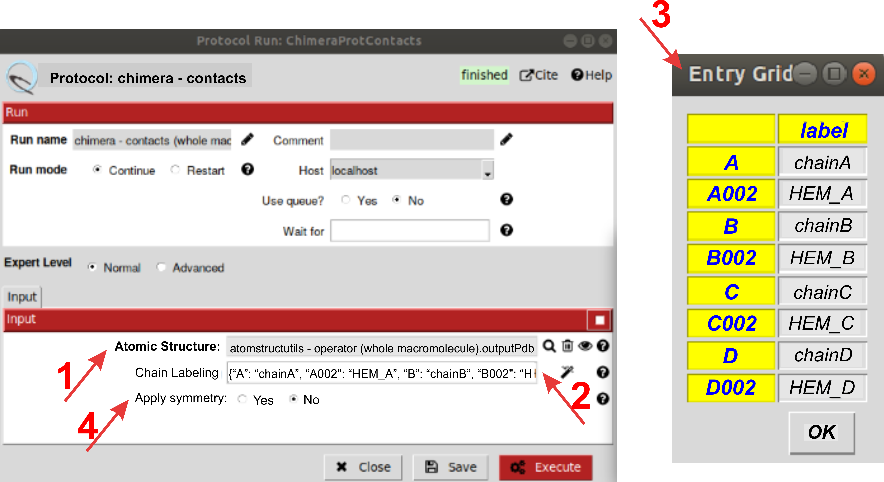
\includegraphics[width=0.85\textwidth]{Images/Fig51}
            \caption{Filling in the \scommand{chimera contacts} protocol form to get all atom contacts between couples of chains within the macromolecule of the human haemoglobin \ttt{metHgb}.}
            \label{fig:contacts_whole_macromolecule}
        \end{figure}
        
 After executing the protocol, resulting contacts can be checked similarly to case A. 
\end{itemize}

\end{comment}

 



















